% *======================================================================*
%  Cactus Thorn template for ThornGuide documentation
%  Author: Ian Kelley
%  Date: Sun Jun 02, 2002
%  $Header$
%
%  Thorn documentation in the latex file doc/documentation.tex
%  will be included in ThornGuides built with the Cactus make system.
%  The scripts employed by the make system automatically include
%  pages about variables, parameters and scheduling parsed from the
%  relevent thorn CCL files.
%
%  This template contains guidelines which help to assure that your
%  documentation will be correctly added to ThornGuides. More
%  information is available in the Cactus UsersGuide.
%
%  Guidelines:
%   - Do not change anything before the line
%       % BEGIN CACTUS THORNGUIDE",
%     except for filling in the title, author, date etc. fields.
%   - You can define your own macros are OK, but they must appear after
%     the BEGIN CACTUS THORNGUIDE line, and do not redefine standard
%     latex commands.
%   - To avoid name clashes with other thorns, 'labels', 'citations',
%     'references', and 'image' names should conform to the following
%     convention:
%       ARRANGEMENT_THORN_LABEL
%     For example, an image wave.eps in the arrangement CactusWave and
%     thorn WaveToyC should be renamed to CactusWave_WaveToyC_wave.eps
%   - Graphics should only be included using the graphix package.
%     More specifically, with the "includegraphics" command. Do
%     not specify any graphic file extensions in your .tex file. This
%     will allow us (later) to create a PDF version of the ThornGuide
%     via pdflatex. |
%   - References should be included with the latex "bibitem" command.
%   - For the benefit of our Perl scripts, and for future extensions,
%     please use simple latex.
%
% *======================================================================*
%
% Example of including a graphic image:
%    \begin{figure}[ht]
% 	\begin{center}
%    	   \includegraphics[width=6cm]{MyArrangement_MyThorn_MyFigure}
% 	\end{center}
% 	\caption{Illustration of this and that}
% 	\label{MyArrangement_MyThorn_MyLabel}
%    \end{figure}
%
% Example of using a label:
%   \label{MyArrangement_MyThorn_MyLabel}
%
% Example of a citation:
%    \cite{MyArrangement_MyThorn_Author99}
%
% Example of including a reference
%   \bibitem{MyArrangement_MyThorn_Author99}
%   {J. Author, {\em The Title of the Book, Journal, or periodical}, 1 (1999),
%   1--16. {\tt http://www.nowhere.com/}}
%
% *======================================================================*

% If you are using CVS use this line to give version information
% $Header$

\documentclass{article}
\bibliographystyle{alpha}

% Use the Cactus ThornGuide style file
% (Automatically used from Cactus distribution, if you have a
%  thorn without the Cactus Flesh download this from the Cactus
%  homepage at www.cactuscode.org)
\usepackage{cactus}

\begin{document}

%%%%%%%%%%%%%%%%%%%%%%%%%%%%%%%%%%%%%%%%%%%%%%%%%%%%%%%%%%%%%%%%%%%%%%%%%%%%%%%%

% The author of the documentation
\author{Jonathan Thornburg \quad {\tt <jthorn@aei.mpg.de>}}

% The title of the document (not necessarily the name of the Thorn)
\title{{\bf AHFinderDirect} -- A Fast Apparent Horizon Finder}

% the date your document was last changed, if your document is in CVS,
% please us:
%    \date{$ $Date$ $}
\date{$ $Date$ $}

\maketitle

% Do not delete next line
% START CACTUS THORNGUIDE

% Add all definitions used in this documentation here
%   \def\mydef etc

%%%%%%%%%%%%%%%%%%%%%%%%%%%%%%%%%%%%%%%%

% misc text stuff
\def\code#1{{\tt #1}}			% variable names, parameter values, etc
\def\defn#1{``#1''}			% definition of a term
\def\arrangement#1{{\bf #1}}		% name of an arrangement
\def\thorn#1{{\bf #1}}			% name of a thorn
\def\program#1{{\bf #1}}		% name of computer program
\def\cvsplace#1{{\bf #1}}		% name of a CVS repository/directory/tag
\def\cf{\hbox{cf.\hbox{}}}
\def\eg{\hbox{eg.\hbox{}}}
\def\ie{\hbox{i.e.\hbox{}}}
\def\eqref#1{$(\ref{#1})$}

% get size/spacing of "++" right, cf online C++ FAQ question 35.1
\def\Cplusplus{\hbox{C\raise.25ex\hbox{\footnotesize ++}}}

% misc math mode stuff
\def\assign{\leftarrow}			% for pseudocode algorithms
\def\ltsim{\lesssim}
\def\gtsim{\gtrsim}
\def\tfrac#1#2{{\textstyle    \frac{#1}{#2}}}
\def\dfrac#1#2{{\displaystyle \frac{#1}{#2}}}
\def\thalf{\tfrac{1}{2}}
\def\const{{\rm const}}
\def\ij{{ij}}
\def\uv{{uv}}
\def\del{\nabla}

\def\I{{\text{\scriptsize I}}}                  % grid-point index
\def\J{{\text{\scriptsize J}}}                  % grid-point index
\def\K{{\text{\scriptsize K}}}                  % grid-point index
\def\M{{\text{\scriptsize M}}}                  % molecule index

\def\Jac[#1]{{\bf J} \bigl[ #1 \bigr]}          % discrete Jacobian for fn #1

% Add an abstract for this thorn's documentation
\begin{abstract}
Thorn \thorn{AHFinderDirect} locates apparent horizons (or more
generally, closed 2-surfaces with $S^2$ topology having any desired
constant expansion) in a numerically computed slice using a direct
method, posing the apparent horizon equation as an elliptic PDE on
angular-coordinate space.  This is very fast and accurate, but
requires a ``reasonable'' initial guess.  This thorn guide describes
how to use the thorn.
\end{abstract}

%%%%%%%%%%%%%%%%%%%%%%%%%%%%%%%%%%%%%%%%%%%%%%%%%%%%%%%%%%%%%%%%%%%%%%%%%%%%%%%%

\section{Introduction}

A \defn{marginally trapped surface} is a closed 2-surface in a slice whose
congruence of future-pointing outgoing null geodesics has zero expansion.
There may be several such surfaces, some nested inside others; an
\defn{apparent horizon} is an outermost marginally trapped surface.
In terms of the usual $3+1$ variables, an apparent horizon satisfies
the equation
\begin{equation}
\Theta \equiv \del_i n^i + K_\ij n^i n^j - K = 0
					\label{AHFinderDirect/eqn-horizon}
\end{equation}
where $n^i$ is the outward-pointing unit normal to the apparent horizon,
and $\del_i$ is the covariant derivative operator associated with the
3-metric $g_\ij$ in the slice.  (See \cite{AHFinderDirect/York89}
for a derivation of equation~\eqref{AHFinderDirect/eqn-horizon}.)
(Optionally, you can replace the right hand side
of~\eqref{AHFinderDirect/eqn-horizon} by any specified nonzero
constant, \ie{} you can find a surface of constant
(in general nonzero) expansion.; this is dicsussed in
section~\ref{AHFinderDirect/sect-parameters/other-parameters}.)

Thorn~\thorn{AHFinderDirect} finds an apparent horizon by numerically
solving equation~\eqref{AHFinderDirect/eqn-horizon}.  It requires
as input the usual Cactus 3-metric $g_\ij$ and extrinsic curvature
$K_\ij$, (and optionally the conformal factor $\psi$ if the
\thorn{StaticConformal} metric semantics are used),
and produces as output the Cactus $(x,y,z)$ coordinates of a large
number of points on the apparent horizon, together with some auxiliary
information like the apparent horizon area and centroid position, and
the irreducable mass associated with the area.

Besides this thorn guide, the other main sources of information on
\thorn{AHFinderDirect} are the comments in the \verb|param.ccl| file,
the paper \cite{AHFinderDirect/Thornburg2003:AH-finding},
and to a lesser extent the paper \cite{AHFinderDirect/Thornburg95}.
As a courtesy, I ask that both these papers be cited in any published
research which uses this thorn, or which uses code from this thorn.

%%%%%%%%%%%%%%%%%%%%%%%%%%%%%%%%%%%%%%%%%%%%%%%%%%%%%%%%%%%%%%%%%%%%%%%%%%%%%%%%

\section{What \thorn{AHFinderDirect} Needs}
\label{AHFinderDirect/sect-what-AHFinderDirect-needs}

There are some restrictions on the spacetime, or more precisely
on each slice where you want to find apparent horizons, which are
necessary in order for \thorn{AHFinderDirect} to work:
\begin{itemize}
\item	\thorn{AHFinderDirect} requires that the Cactus geometry
	($g_{ij}$, $K_{ij}$, and optionally $\psi$) be nonsingular
	in a neighborhood of the apparent horizon.  In particular,
	this means that it quite certainly will {\em not\/} work for
	spacetimes/slicings which have a singular geometry on the
	horizon, such as Schwarzschild/Schwarzschild and
	Kerr/Boyer-Lindquist.%%%
\footnote{%%%
	 Nonsingular slicings of those same spacetimes,
	 such as Schwarzschild/Eddington-Finkelstein,
	 Kerr/Kerr, and Kerr/Kerr-Schild, are fine, and
	 are in fact nice test cases.
	 }%%%
\item	Less obviously, this also means that if there is a
	singularity in the geometry somewhere near the apparent
	horizon, then you need to have a high enough Cactus 3-D grid
	resolution that the geometry interpolation doesn't ``see''
	the singularity.  (If \thorn{AHFinderDirect} ``sees'' the
	singularity, it may ``just'' fail to find the horizon,
	and/or it may report that the interpolated $g_{ij}$ fails
	to be positive definite or even contains NaNs.)
\item	At the moment \thorn{AHFinderDirect} and the Cactus interpolators
	don't know how to avoid an excised region, so if the apparent horizon
	(or any trial horizon surface as the algorithm is iterating
	towards the apparent horizon) gets too close to an excised
	region, you'll get garbage results as the interpolator tries
	to interpolate data from the excised region.  I plan to fix
	this sometime soon.
\item	\thorn{AHFinderDirect} requires that any apparent horizon
	it's going to (try to) find must be a \defn{Strahlk\"{o}rper}
	(literally ``ray body'', or more commonly ``star-shaped region'')
	relative to some local coordinate origin (which you must specify).
	A Strahlk\"{o}rper is defined by Minkowski
	(\cite[p.~108]{AHFinderDirect/Schroeder86})
	as
	   \begin{quote}
	   a region in $n$-dimensional Euclidean space containing the
	   origin and whose surface, as seen from the origin, exhibits
	   only one point in any direction.
	   \end{quote}
	In other words, using polar spherical coordinates relative
	to the local coordinate origin, the apparent horizon's shape
	must be parameterizable as $r = h(\text{angle})$ for some
	single-valued function $h: S^2 \to \Re^+$.  (\thorn{AHFinderDirect}
	uses precisely this parameterization.)
\end{itemize}

There are also some restrictions on your Cactus configuration and run;
here's what works and what doesn't:
\begin{itemize}
\item	I {\em strongly\/} recommend using a current-CVS checkout of
	the Cactus flesh and of all relevant thorns.  I haven't tested
	\thorn{AHFinderDirect} at all with older versions of the flesh
	or other thorns.
\item	\thorn{AHFinderDirect} works fine with the \thorn{PUGH} unigrid
	driver and with the \thorn{Carpet} mesh-refinement driver.  So
	far as I know it's never been tested with any other driver.
\item	\thorn{AHFinderDirect} works fine in single- or multi-processor
	Cactus runs.
\item	Obviously, your Cactus configuration must include
	\thorn{AHFinderDirect}, and your \code{ActiveThorns} parameter(s)
	must activate it.
\item	\thorn{AHFinderDirect} inherits from the other thorns
	(strictly speaking, implementations) listed in
	table~\ref{AEIThorns/AHFinderDirect/tab-inherits-from},
	so you'll need them (or more precisely some thorns providing them)
	in your configuration and activated, too.


%%%%%%%%%%%%%%%%%%%%%%%%%%%%%%%%%%%%%%%%
\begin{table}[tbp]
\begin{center}
\begin{tabular}{l@{\qquad}l}
\thorn{Implementation}		& Typically provided by \thorn{Thorn}	\\
\hline %---------------------------------------------------------------
\thorn{Grid}			& \thorn{CactusBase/CartGrid3d}		\\
\thorn{IO}			& \thorn{CactusBase/IOUtil}		\\
\thorn{ADMBase}			& \thorn{CactusEinstein/ADMBase}	\\
\thorn{StaticConformal}		& \thorn{CactusEinstein/StaticConformal}\\
\thorn{SpaceMask}		& \thorn{CactusEinstein/SpaceMask}	\\
\thorn{SphericalSurface}	& \thorn{AEIThorns/SphericalSurface}	%%%\\
\end{tabular}
\end{center}
\caption[Other Thorns from which \thorn{AHFinderDirect} Inherits]
	{
	This table lists all the other implementations from which
	\thorn{AHFinderDirect} inherits, and the thorns which typically
	provide these implementations.
	}
\label{AEIThorns/AHFinderDirect/tab-inherits-from}
\end{table}
%%%%%%%%%%%%%%%%%%%%%%%%%%%%%%%%%%%%%%%%

\item	\verb|Grid::domain = "full"|, \verb|"bitant"|,
	\verb|"quadrant"|, and \verb|"octant"| are supported.
	Alas, at present rotating (or more precisely nonlocal)
	symmetry boundary conditions aren't supported.
\item	The \verb|ADMBase::metric_type| values \verb|"physical"| and
	\verb|"static conformal"| are supported; for the latter you must
	have storage turned on for at least the conformal factor
	\verb|StaticConformal::psi|.  (The Cactus 3-D grid functions
	for 1st and 2nd derivatives of \verb|psi| aren't used.)
\item	\thorn{AHFinderDirect} uses the \verb|CCTK_InterpGridArrays()|
	Cactus global (multi-processor grid array) interpolator API;
	this is provided by \thorn{PUGHInterp} or \thorn{CarpetInterp}
	(so you must have the appropriate one of these thorns compiled
	in and activated).  \verb|CCTK_InterpGridArrays()| in turn uses
	the new \verb|CCTK_InterpLocalUniform()| processor-local
	interpolator API; \thorn{AHFinderDirect} uses various options
	in this API which at present are only supported by thorn
	\thorn{AEILocalInterp} (so you must have this thorn compiled in
	and activated)
\item	\thorn{AHFinderDirect} uses various Cactus reduction APIs to
	coordinate multi-processor horizon finding, so (even if you're
	only going to run on a single processor) you must have a reduction
	thorn like \thorn{PUGHReduce} or \thorn{CarpetReduce} compiled in
	and activated.
\item	At present only a few of \thorn{AHFinderDirect}'s parameters
	are steerable.  (This is actually quite easy to fix; I just
	haven't gotten around to it yet.)
\item	I think \thorn{AHFinderDirect} will ``work'' with checkpoint/restart,
	but I haven't tested this yet.  Here ``work'' means the restart
	will be like starting a new run, in that \thorn{AHFinderDirect}
	will set the initial guess for each horizon in a start-of-a-new-run
	manner.  Alas, it will also write a new \verb|BH_diagnostics| file
	for each horizon found, overwriting any existing \verb|BH_diagnostics|
	files.  This is a bug, which I plan to fix soon (the right behavior
	is/will be to {\em append\/} to the existing \verb|BH_diagnostics|
	file).
\end{itemize}

\thorn{AHFinderDirect} can pass information to the rest of Cactus in
several ways; these are described in detail in
section~\ref{AHFinderDirect/sect-parameters/communicating-with-other-thorns}.

%%%%%%%%%%%%%%%%%%%%%%%%%%%%%%%%%%%%%%%%%%%%%%%%%%%%%%%%%%%%%%%%%%%%%%%%%%%%%%%%

\section{Obtaining and Compiling \thorn{AHFinderDirect}}

You should be able to obtain the source code for this thorn via the
usual procedures for anonymous git checkout; at present it lives in
the \arrangement{EinsteinAnalysis} arrangement.

This thorn is written primarily in \Cplusplus{}, calling C and
Fortran~77 numerical libraries.%%%
\footnote{%%%
	 The (C) code for the relativity computations
	 (\ie{}~the apparent horizon equation itself)
	 is mainly machine-generated from Maple code,
	 which in turn uses a Perl preprocessor.
	 But the machine-generated C code is already
	 in CVS along with the rest of this thorn's
	 source code, so you don't need to have Maple
	 installed unless you want to modify the
	 relativity computations.%%%
	 }%%%
{}  In theory the code should be quite portable to modern \Cplusplus{}
compilers, but in practice I've had a number of portability problems
with various compilers.  See the ``Code Notes'' and ``Compiler Notes''
sections in the top-level \code{README} file for details and lists of
compilers currently known to be ok or not.

By default \thorn{AHFinderDirect} doesn't use any external libraries.
However, if \code{HAVE\_DENSE\_JACOBIAN\_\_LAPACK} is defined in
\code{src/include/config.h}, then \thorn{AHFinderDirect} uses the
LAPACK library for solving linear equations.  In this case you need
to configure Cactus with \code{LAPACK=yes}.  See the top-level
\code{README} and \code{README.library} files for details on this.

%%%%%%%%%%%%%%%%%%%%%%%%%%%%%%%%%%%%%%%%%%%%%%%%%%%%%%%%%%%%%%%%%%%%%%%%%%%%%%%%

\section{\thorn{AHFinderDirect} Parameters}

This thorn has lots of parameters, but most of them have reasonable
default values which you probably won't need to change.  Here I describe
the parameters which you are likely to want to at least look at, and
possibly set explicitly.

Note that all of the ``\code{[}$n$\code{]}'' parameters are Cactus
array parameters, which you need to specify separately in your parameter
file for each apparent horizon.  {\bf IMPORTANT: Apparent horizons are
numbered starting at 1, not 0!}  The example in
section~\ref{AHFinderDirect/sect-examples} should make this clear.

%%%%%%%%%%%%%%%%%%%%%%%%%%%%%%%%%%%%%%%%

\subsection{Overall Parameters}
\label{AHFinderDirect/sect-parameters/overall-parameters}

\begin{description}
\item[\code{find\_every}]
\mbox{}\\
	This is an integer parameter specifying how often
	\thorn{AHFinderDirect} should try to find apparent horizons:
	If $\verb|find_every| = 0$, \thorn{AHFinderDirect} is a no-op.
	If $\verb|find_every| \ne 0$, \thorn{AHFinderDirect} tries to
	find apparent horizons each \verb|find_every| time steps.%%%
\footnote{%%%
	 More precisely, if ${\tt find\_every} \ne 0$,
	 \thorn{AHFinderDirect} tries to find apparent
	 horizons at each time step where {\tt cctk\_iteration}
	 is evenly divisible by {\tt find\_every}.
	 }%%%
{}	The default value is~1, \ie{} \thorn{AHFinderDirect} tries
	to find apparent horizons at every time step.
\item[\code{N\_horizons}]
\mbox{}\\
	How many apparent horizons do you want to find in each slice?
	Typical values are 1 (the default), 2, or 3.%%%
\footnote{%%%
	 Larger values are also possible.  The present upper
	 limit is 100, but it would be trivial to raise this
	 further if desired -- see the comments in \code{param.ccl}
	 for details.
	 }%%%
{}	{\bf This thorn numbers the apparent horizons from 1 to
	\code{N\_horizons} inclusive.}
	There are a number of other parameters (described below)
	which you need to set for of these each apparent horizons.

	Note that \code{N\_horizons} sets the number of apparent horizons
	you want to find {\em in the Cactus 3-D numerical grid\/}, not in
	the whole spacetime.  For example, if you are simulating (say)
	Misner data with \verb|Grid::domain = "bitant"|, with the two
	throats at (say) roughly $z = \pm 1$, then you should set
	\verb|N_horizons = 1| to find those two apparent horizons,
	since you're only finding one apparent horizon within the
	numerical grid.  If you also want to search for a common
	apparent horizon surrounding both black holes, then you should
	set \verb|N_horizons = 2|, since you're finding at most 2
	apparent horizons within the numerical grid.

\item[\code{verbose\_level}]
\mbox{}\\
	This controls how verbose this thorn is in printing
	informational (non-error) messages describing what it's
	doing.  In order from tersest to most verbose, the allowable
	values are
	\begin{description}
	\item[\code{"no output"}]
	\mbox{}\\
		Don't print anything.
	\item[\code{"physics highlights"}]
	\mbox{}\\
		Print only a single line each time
		\thorn{AHFinderDirect} runs, giving which
		horizons were found.
	\item[\code{"physics details"}]
	\mbox{}\\
		Print two lines for each horizon found, giving
		the horizon area, centroid position, and irreducible mass.
		This is the default.
	\item[\code{"algorithm highlights"}]
	\mbox{}\\
		Also print a single line for each Newton iteration giving
		the 2-norm and $\infty$-norm of the $\Theta(h)$ function
		defined by equation~\eqref{AHFinderDirect/eqn-horizon}.
	\item[\code{"algorithm details"}]
	\mbox{}\\
		Print lots of detailed messages tracing what the code
		is doing.
	\item[\code{"algorithm debug"}]
	\mbox{}\\
		Print even more detailed messages tracing what the code
		is doing, mainly useful for debugging purposes.
	\end{description}
\end{description}

%%%%%%%%%%%%%%%%%%%%%%%%%%%%%%%%%%%%%%%%

\subsection{Choosing the Local Coordinate Origin for each Apparent Horizon}
\label{AHFinderDirect/sect-parameters/local-coordinate-origin}

For each apparent horizon you want to find, you need to specify
the Cactus $(x,y,z)$ coordinates of a local coordinate system origin.
As described in
section~\ref{AHFinderDirect/sect-what-AHFinderDirect-needs},
each apparent horizon must be a Strahlk\"{o}rper with respect to its
local coordinate system origin.

You specify the local coordinate system origin for each horizon with
the (Cactus array) parameters
\begin{description}
\item[%%%
     \begin{tabular}{@{}l@{}}
     \code{origin\_x[}$n$\code{]}	\\
     \code{origin\_y[}$n$\code{]}	\\
     \code{origin\_z[}$n$\code{]}	%%%\\
     \end{tabular}
     ]
\mbox{}\\
	These all default to 0.0.
	In practice, you should set these parameters to be somewhere
	reasonably close to your best guess for the center of each apparent
	horizon.  These aren't {\em too\/} critical: being off by 1/4
	of the horizon radius is no problem, and -- assuming the algorithm
	still converges -- even 1/2 of the horizon radius only slows
	the convergence by an extra iteration or two.  But poor values
	of these parameters do make the algorithm more likely to fail
	to converge.
\end{description}

At present the local coordinate origin is fixed once you set it;
there's no provision for it to move to track a moving black hole.
I hope to add such a provision soon.%%%
\footnote{%%%
	 This would be along the lines of the
	 \thorn{AHFinder} apparent horizon finder's
	 \code{AHFinder::ahf\_wander = true}
	 option.
	 }%%%

%%%%%%%%%%%%%%%%%%%%%%%%%%%%%%%%%%%%%%%%

\subsection{Specifying the Initial Guess}

\thorn{AHFinderDirect} requires an initial guess
for the apparent horizon's coordinate position and shape
(that is, for the $h(\text{angle})$ function defined in
section~\ref{AHFinderDirect/sect-what-AHFinderDirect-needs}),
for each apparent horizon you want to find.  Unlike some other apparent
horizon finders (\eg{}~the curvature flow method in \thorn{AHFinder}),
for \thorn{AHFinderDirect} there's no restriction on whether the initial
guess is inside, outside, or crossing the actual apparent horizon: the
only important thing is that it should be ``close''.  Just how close
the initial guess needs to be for \thorn{AHFinderDirect} to find the
(a) apparent horizon depends on the slice and the coordinates, but as
a general rule of thumb any initial guess that's within 1/3 to 1/2 of
the mean horizon radius will probably work.

The ``initial guess'' specification is used the first time we try to
find any given apparent horizon, and also any succeeding time when the
most recent attempt to find this apparent horizon failed.  If we succeed
in finding a given apparent horizon, than that apparent horizon position
is automatically reused as the initial guess the next time we try to
find the same apparent horizon; in this case the explicit ``initial guess''
specification is ignored.%%%
\footnote{%%%
	 This is similar to the \thorn{AHFinder} apparent
	 horizon finder's behavior with the
	 \code{AHFinder::ahf\_guessold = true}
	 option.
	 }%%%

There are a number of parameters for specifying the initial guess:
\begin{description}
\item[\code{initial\_guess\_method[}$n$\code{]}]
\mbox{}\\
	This sets what type of the initial guess is used for each
	apparent horizon position.
	There are several possibilities, most with their own sets
	of subparameters:%%%
\footnote{%%%
	 The naming scheme for these is similar to
	 that used in the \thorn{Exact} thorn.
	 }%%%
$^,$%%%
\footnote{%%%
	 For the Kerr parameters, note that this thorn
	 always uses the convention that the spin parameter
	 $a \equiv J/m^2$ is dimensionless.
	 }%%%
	\begin{description}
	\item[\code{"read from file"}]
	\mbox{}\\
		This reads the initial-guess $h(\text{angle})$ function
		from a data file.  The file format is currently hard-wired
		to be that written with \verb|file_format = "ASCII (gnuplot)"|
		(see below).  The subparameter
		\verb|initial_guess__read_from_named_file__file_name|
		specifies the file name.
	\item[\code{"Kerr/Kerr"}]
	\mbox{}\\
		This sets the initial guess to the analytically-known
		apparent horizon position in a Kerr spacetime
		in Kerr coordinates.  This is a coordinate sphere
		of radius $(1 + \sqrt{1 - a^2}) m$.
		There are subparameters
		\begin{description}
		\item[%%%
		     \begin{tabular}{@{}l@{}}
		     \code{initial\_guess\_\_Kerr\_Kerr\_\_x\_posn[}$n$\code{]} \\
		     \code{initial\_guess\_\_Kerr\_Kerr\_\_y\_posn[}$n$\code{]} \\
		     \code{initial\_guess\_\_Kerr\_Kerr\_\_z\_posn[}$n$\code{]} %%%\\
		     \end{tabular}%%%
		     ]
		\mbox{}\\
			to set the position of the Kerr black hole
			(note this position is in {\em global\/} Cactus
			coordinates, not relative to the local coordinate
			origin), and
		\item[%%%
		     \begin{tabular}{@{}l@{}}
		     \code{initial\_guess\_\_Kerr\_Kerr\_\_mass[}$n$\code{]} \\
		     \code{initial\_guess\_\_Kerr\_Kerr\_\_spin[}$n$\code{]} %%%\\
		     \end{tabular}%%%
		     ]
		\mbox{}\\
			to set its mass and spin.
		\end{description}
	\item[\code{"Kerr/Kerr-Schild"}]
	\mbox{}\\
		This sets the initial guess to the analytically-known
		apparent horizon position in a Kerr spacetime in
		Kerr-Schild coordinates.  This is a coordinate ellipsoid
		with radia (semi-major axes)
		\begin{equation}
		\renewcommand{\arraystretch}{2.0}
		\begin{array}{lclcl}
		r_z	& = &	(1 + \sqrt{1 - a^2}) m			\\
		r_x = r_y
			& = &	r_z \sqrt{1 + \left(\dfrac{am}{r_z}\right)^2}
			& = &	\sqrt{\dfrac{2 r_z}{m}} \, m
									%%%\\
		\end{array}
		\end{equation}
		\begin{description}
		\item[%%%
		     \begin{tabular}{@{}l@{}}
		     \code{initial\_guess\_\_Kerr\_KerrSchild\_\_x\_posn[}$n$\code{]} \\
		     \code{initial\_guess\_\_Kerr\_KerrSchild\_\_y\_posn[}$n$\code{]} \\
		     \code{initial\_guess\_\_Kerr\_KerrSchild\_\_z\_posn[}$n$\code{]} %%%\\
		     \end{tabular}%%%
		     ]
		\mbox{}\\
			(note this position is in {\em global\/} Cactus
			coordinates, not relative to the local coordinate
			origin), and
		\item[%%%
		     \begin{tabular}{@{}l@{}}
		     \code{initial\_guess\_\_Kerr\_KerrSchild\_\_mass[}$n$\code{]} \\
		     \code{initial\_guess\_\_Kerr\_KerrSchild\_\_spin[}$n$\code{]} %%%\\
		     \end{tabular}%%%
		     ]
		\mbox{}\\
			to set its mass and spin.
		\end{description}
	\item[\code{"coordinate sphere"}]
	\mbox{}\\
		This sets the initial guess to a coordinate sphere;
		there are subparameters
		\begin{description}
		\item[%%%
		     \begin{tabular}{@{}l@{}}
		     \code{initial\_guess\_\_coord\_sphere\_\_x\_center[}$n$\code{]} \\
		     \code{initial\_guess\_\_coord\_sphere\_\_y\_center[}$n$\code{]} \\
		     \code{initial\_guess\_\_coord\_sphere\_\_z\_center[}$n$\code{]} %%%\\
		     \end{tabular}%%%
		     ]
		\mbox{}\\
			(note this position is in {\em global\/} Cactus
			coordinates, not relative to the local coordinate
			origin), and
		\item[\code{initial\_guess\_\_coord\_sphere\_\_radius[}$n$\code{]}]
		\mbox{}\\
			to set the radius.
		\end{description}
	\item[\code{"coordinate ellipsoid"}]
	\mbox{}\\
		This sets the initial guess to a coordinate ellipsoid;
		there are subparameters
		\begin{description}
		\item[%%%
		     \begin{tabular}{@{}l@{}}
		     \code{initial\_guess\_\_coord\_ellipsoid\_\_x\_center[}$n$\code{]} \\
		     \code{initial\_guess\_\_coord\_ellipsoid\_\_y\_center[}$n$\code{]} \\
		     \code{initial\_guess\_\_coord\_ellipsoid\_\_z\_center[}$n$\code{]} %%%\\
		     \end{tabular}%%%
		     ]
		\mbox{}\\
			(note this position is in {\em global\/} Cactus
			coordinates, not relative to the local coordinate
			origin), and
		\item[%%%
		     \begin{tabular}{@{}l@{}}
		     \code{initial\_guess\_\_coord\_ellipsoid\_\_x\_radius[}$n$\code{]}	\\
		     \code{initial\_guess\_\_coord\_ellipsoid\_\_y\_radius[}$n$\code{]}	\\
		     \code{initial\_guess\_\_coord\_ellipsoid\_\_z\_radius[}$n$\code{]}	%%%\\
		     \end{tabular}%%%
		     ]
		\mbox{}\\
			to set the radia (semimajor axes).
		\end{description}
	\end{description}
\end{description}

%%%%%%%%%%%%%%%%%%%%%%%%%%%%%%%%%%%%%%%%

\subsection{I/O Parameters for the Apparent Horizon Shape(s)}

The main output of this thorn is the computed horizon shape function
$h({\rm angle})$, and correspondingly the $(x,y,z)$ coordinate positions
of the apparent-horizon-surface (angular) grid points.  There are several
parameters controlling if, how often, and how these should be written
to data files:

\begin{description}
\item[\code{output\_h\_every}]
\mbox{}\\
	As described in
	section~\ref{AHFinderDirect/sect-parameters/overall-parameters},
	\thorn{AHFinderDirect} will try to find the apparent horizon(s)
	every \verb|find_every| time steps.  However, you can control
	how often (if at all) the apparent horizon shape(s) are written
	to data files: this is only done if \verb|output_h_every|
	is nonzero, and the Cactus time step number \verb|cctk_iteration|
	is an integral multiple of this parameter (\verb|output_h_every|).

\item[\code{file\_format}]
\mbox{}\\
	This specifies the file format for horizon-shape (and other
	angular-grid-function) data files.  Unfortunately, at the
	moment only a single format is implemented,
	\begin{description}
	\item[\code{"ASCII (gnuplot)"}]
	\mbox{}\\
		This is a simple ASCII format designed for easy
		plotting with gnuplot:
		\begin{itemize}
		\item	\thorn{AHFinderDirect} writes a separate data file
			for each Cactus time step and for each apparent
			horizon found.  By default these are all written
			in to the \verb|IOUtil::out_dir| directory;
			see \verb|h_directory| (below) to change this.
		\item	The time step number and the apparent horizon number
			are both encoded in the file name; the actual
			file name is given by a \verb|printf()| format
			\verb|"%s/%s.t%d.ah%d.%s"|, where
			\begin{itemize}
			\item	the first \verb|%s| is the directory
				set by the \verb|IO::out_dir| and/or
				\verb|h_directory| parameters (see below)
			\item	the second \verb|%s| is the base file name
				set by the \verb|h_base_file_name|
				parameter (see below)
			\item	the first \verb|%d| is the
				Cactus time step number
			\item	the second \verb|%d| is the
				apparent horizon number
			\item	the third \verb|%s| is the
				file name extension, set by the
				\verb|ASCII_gnuplot_file_name_extension|
				parameter; this defaults to \verb|"gp"|
			\end{itemize}
		\item	Comment lines begin with \verb|#|.
		\item	Patches are separated by 2 blank lines;
			rows of apparent-horizon points within a patch
			are separated by single blank lines.
		\item	Each apparent-horizon-surface point
			is described by a single line, containing
			the whitespace-separated fields
			\begin{itemize}
			\item	Two ``unwrapped'' angular coordinates
				in degrees, representing a point on $S^2$.
			\item	The $h$ value, giving the radius
				of the apparent horizon surface
				at that angle.
			\item	The corresponding Cactus $(x,y,z)$
				coordinates.
			\end{itemize}
		\end{itemize}
		See section~\ref{AHFinderDirect/sect-visualization}
		for a discussion of visualization for these and other
		\thorn{AHFinderDirect} output files.
	\end{description}

\item[\code{h\_directory}]
\mbox{}\\
	This specifies the directory in which the $h$ data files
	are to be written.  If it doesn't already exist, this directory
	is created before writing the data files.  This parameter
	defaults to the value of the \verb|IO::out_dir| parameter.

\item[\code{h\_base\_file\_name}]
\mbox{}\\
	This specifies the base file name for $h$ data files, as
	described above.  This defaults to "h".

\item[\code{ASCII\_gnuplot\_file\_name\_extension}]
\mbox{}\\
	This specifies the file name extension for $h$ data files, as
	described above.  This defaults to "gp".
\end{description}

%%%%%%%%%%%%%%%%%%%%%%%%%%%%%%%%%%%%%%%%

\subsection{Parameters for the ``BH\_diagnostics'' Files}
\label{AHFinderDirect/sect-parameters/BH-diagnostics-parameters}

As well as the apparent horizon shape files, this thorn can also
write files giving time series of various diagnostics.  These are
controlled by the following parameters:

\begin{description}
\item[\code{output\_BH\_diagnostics}]
\mbox{}\\
	If this Boolean parameter is set to true,
	\thorn{AHFinderDirect} will write a ``black hole diagnostics''
	file for each distinct apparent horizon found
	(up to \verb|N_horizons| files in all).  Each such file
	contains a time series of various diagnostics for all time
	steps when the corresponding apparent horizon was found.
	The file format is again a simple ASCII format designed
	for easy plotting with gnuplot:
	\begin{itemize}
	\item	The apparent horizon number is encoded in the file name;
		the actual file name is given by a \verb|printf()| format
		\verb|"%s/%s.ah%d.%s"|, where
		\begin{itemize}
		\item	the first \verb|%s| is the directory
			set by the \verb|IO::out_dir| and/or
			\verb|BH_diagnostics_directory| parameters (see below)
		\item	the second \verb|%s| is the base file name
			set by the \verb|BH_diagnostics_base_file_name|
			parameter (see below); this defaults to
			\verb|"BH_diagnostics"|
		\item	the \verb|%d| is the apparent horizon number
		\item	the third \verb|%s| is the file name extension,
			set by the \verb|BH_diagnostics_file_name_extension|
			parameter; this defaults to \verb|"gp"|
		\end{itemize}
	\item	The file begins with a block of header comments
		(lines begining with \verb|#|) describing the data
		fields.
	\item	Each time this apparent horizon is found, a single
		line is appended to the data file, containing various
		whitespace-separated fields.  The the precise list of
		fields, see the header comments, or see the function
		\verb|output()| in \verb|src/driver/BH_diagnostics.cc|.
		As of this writing the fields are:
		\begin{itemize}
		\item	the Cactus iteration number \verb|cctk_iteration|
		\item	the Cactus time coordinate \verb|cctk_time|
		\item	the Cactus $(x,y,z)$ coordinates of the apparent
			horizon centroid
		\item	the minimum, maximum, and mean coordinate radia
			of the apparent horizon about the local
			coordinate origin
		\item	the minimum and maximum Cactus $x$, $y$, and $z$
			coordinates of the apparent horizon surface
		\item	the proper circumferences of the apparent horizon
			in the $xy$, $xz$, and $yz$ local-coordinate planes%%%
\footnote{%%%
	 Note that if the apparent horizon is not
	 symmetric across one of these coordinate planes,
	 then the circumference in this plane is not
	 very meaningful.  In particular, in this case
	 this circumference is probably different from
	 the apparent horizon's maximum ``hoop'' circumference.
	 }%%%
		\item	the $xz/xy$ and $yz/xy$ ratios of the proper
			circumferences
		\item	the proper area of the apparent horizon, $A$
		\item	the irreducible mass of the apparent horizon,
			$\sqrt{A/16\pi}$
		\item	the areal radius of the apparent horizon,
			$\sqrt{A/4\pi}$
		\end{itemize}
	\end{itemize}

\item[\code{BH\_diagnostics\_directory}]
\mbox{}\\
	This specifies the directory in which the black hole diagnostics
	data files are to be written.  If it doesn't already exist, this
	directory is created before writing the data files.  This parameter
	defaults to the value of the \verb|IO::out_dir| parameter.

\item[\code{BH\_diagnostics\_base\_file\_name}]
\mbox{}\\
	This specifies the base file name for black hole diagnostics
	data files, as described above.  This defaults to
	\verb|"BH_diagnostics"|.

\item[\code{BH\_diagnostics\_file\_name\_extension}]
\mbox{}\\
	This specifies the file name extension for black hole diagnostics
	data files, as described above.  This defaults to \verb|"gp"|.
\end{description}

%%%%%%%%%%%%%%%%%%%%%%%%%%%%%%%%%%%%%%%%

\subsection{(Excision) Mask Parameters}
\label{AHFinderDirect/sect-parameters/mask-parameters}

This thorn can optionally set a mask grid function (or functions)
at each point of the Cactus grid, to indicate where that point is
with respect to the apparent horizon(s).  This is usually used for
excision.

\begin{description}
\item[%%%
     \begin{tabular}{@{}l@{}}
     \code{set\_mask\_for\_all\_horizons}			\\
     \code{set\_mask\_for\_individual\_horizon[}$n$\code{]}	%%%\\
     \end{tabular}
     ]
\mbox{}\\
	These Boolean parameters control whether \thorn{AHFinderDirect}
	should set a mask grid function(s): If the (C) expression
	\verb:set_mask_for_all_horizons || set_mask_for_individual_horizon[i]:
	is true, then \thorn{AHFinderDirect} will set a mask grid
	function(s) for apparent horizon $i$.
	All these parameters default to false (don't set a mask).

	If any of these parameters is set to true, you almost certainly
	also need to set the Boolean parameter \verb|SpaceMask::use_mask|
	to true to to turn on storage for the mask grid function(s)!
\end{description}

If it's setting a mask(s), \thorn{AHFinderDirect} partitions the
Cactus grid into 3~regions: an \defn{inside}, a \defn{buffer},
and an \defn{outside}.  Typically the inner region is excised, but
\thorn{AHFinderDirect} doesn't itself do this:  It just sets the mask(s);
you need to use some other thorn(s) to do the actual excision.

The 3~regions are defined as follows:  For a grid point a distance $r[i]$
from horizon~$i$'s local coordinate origin, with horizon~$i$'s radius
in this same direction (again, measured from its local coordinate origin)
being $r_{\text horizon}[i]$,%%%
\footnote{%%%
	 Note that these are flat-space distances
	 $[(x-x_0)^2 + (y - y_0)^2 + (z-z_0)^2]^{1/2}$
	 -- the spacetime metric is {\em not\/} used here.
	 }%%%
{} the regions are defined by
\begin{equation}
\renewcommand{\arraystretch}{1.333}
\begin{tabular}{l@{~}lll@{~}lll}
$r[i] \le r{	ext{r}}[i]$	& \text{for some $i$}
	&
	&				&
	& $\Rightarrow$	& \text{inner}					\\
$r[i] >   r_{\text{r}}[i]$	& \text{for all $i$}
	& \text{and}	&
	$r[i] \le r_{\text{r}}[i]$	& \text{for some $i$}
	& $\Rightarrow$	& \text{buffer}					\\
$r[i] >   r_{\text{r}}[i]$	& \text{for all $i$}
	&
	&				&
	& $\Rightarrow$	& \text{outer}				%%%\\
\end{tabular}
\end{equation}
where
\begin{equation}
\renewcommand{\arraystretch}{1.333}
\begin{array}{lcl}
r_{\text{r}}
	& = &	\verb|mask_radius_multiplier| \times r_{\text{n}}
		\,\,+\,\,
		\verb|mask_radius_offset| \times {\Delta x}_{\text{e}}
									\\
r_{\text{r}}
	& = &	r_{\text{r}}
		\,\,+\,\,
		\verb|mask_buffer_thickness| \times {\Delta x}_{\text{e}}
									%%%\\
\end{array}
				\label{AHFinderDirect/eqn-r-inside-outside}
\end{equation}
and where ${\Delta x}_{\text{e}}$ is the base-grid Cactus grid spacing
(more precisely, the geometric mean of the base grid's $x$, $y$,
and $z$ Cactus grid spacings)%%%
\footnote{%%%
	 The ``base grid'' part here only matters if
	 you're doing mesh refinement, in which case
	 it's necessary to keep excision consistent
	 between the different refinement levels.
	 }%%%
.

\begin{description}
\item[%%%
     \begin{tabular}{@{}l@{}}
     \code{mask\_radius\_multiplier}	\\
     \code{mask\_radius\_offset}	\\
     \code{mask\_buffer\_thickness}	%%%\\
     \end{tabular}
     ]
\mbox{}\\
	These parameters are used to define the radia $r_{\text{r}}$
	and $r_{\text{r}}$ in
	equation~\eqref{AHFinderDirect/eqn-r-inside-outside} above.

	Note that the sign convention here is that
	\verb|mask_radius_multiplier| is {\em multiplied\/}
	by the horizon radius, then \verb|mask_radius_offset|
	(scaled by the Cactus grid spacing) is {\em added\/}.
	Thus for use with excision (where the inner region --
	which will be excised -- must be somewhat {\em inside\/}
	the horizon), \verb|mask_radius_multiplier| should be a
	positive real number slightly less than~1.0, and/or
	\verb|mask_radius_offset| a negative real number.

	The default values for these parameters are
	\begin{verbatim}
	mask_radius_multiplier =  0.8
	mask_radius_offset     = -5.0
	mask_buffer_thickness  =  5.0
	\end{verbatim}

\item[\code{mask\_is\_noshrink}]
\mbox{}\\
	This Boolean parameter specifies whether the inside and
	buffer regions should be prevented from ever shrinking
	during a time evolution (this is the default), or whether
	they should be set independently from one time step to the
	next (and thus allowed to either grow or shrink).  More
	precisely, once a given grid point has been classified as
	inside, buffer, or outside, \thorn{AHFinderDirect} executes
	the following algorithm:
	\begin{description}
	\item[inside]\mbox{}\\[-\baselineskip]
		\begin{tabbing}
		$\verb|mask| \assign \verb|inside_value|$		  %%%\\
		\end{tabbing}
	\item[buffer]\mbox{}\\[-\baselineskip]
		\begin{tabbing}
		if \=(\verb|mask_is_noshrink|
		      \verb|&&|
		      ($\verb|mask| = \verb|inside_value|$))		\+\\
		   then \=\{						\+\\
			\verb|#|
			this point was previously {\bf inside}
			$\Rightarrow$ no-op here			  \\
			\}						\-\\
		   else \>$\verb|mask| \assign \verb|buffer_value|$	\-%%%\\
		\end{tabbing}
	\item[outside]\mbox{}\\[-\baselineskip]
		\begin{tabbing}
		if \=(\verb|mask_is_noshrink|
		      \verb|&&|
		      (($\verb|mask| = \verb|inside_value|$)
		       \verb.||. ($\verb|mask| = \verb|buffer_value|$))	\+\\
		   then \=\{						\+\\
			\verb|#|
			this point was previously {\bf inside}
			or {\bf buffer} $\Rightarrow$ no-op here	  \\
			\}						\-\\
		   else \>$\verb|mask| \assign \verb|outside_value|$	\-%%%\\
		\end{tabbing}
	\end{description}

\item[\code{min\_horizon\_radius\_points\_for\_mask}]
\mbox{}\\
	By default, \thorn{AHFinderDirect} sets the mask for each
	apparent horizon found.  If we're using mesh refinement, it's
	possible for an apparent horizon to be found on a coarse grid,
	and the masked region to be only a few grid points across on
	a fine grid.  This causes some other Cactus thorns
	(\eg{} \thorn{LegoExcision}) to crash. :(

	This parameter can be used to avoid this problem:
	For each apparent horizon that it finds, \thorn{AHFinderDirect}
	only sets the mask on a given grid if
	\begin{equation}
	r_{\text{inner},\min} \ge \verb|min_horizon_radius_points_for_mask|
		     * {\Delta x}_{\text{current},\max}
	\end{equation}
	where $r_{\text{inner},\min}$ is the minimum over all angles
	of $r_{\text{r}}$ as defined by
	equation~\eqref{AHFinderDirect/eqn-r-inside-outside},
	and ${\Delta x}_{\text{current},\max}$ is the maximum of the
	Cactus $x$, $y$, and~$z$ grid spacings on the current Cactus
	grid.%%%
\footnote{%%%
	 Note that this is the {\bf current\/} Cactus
	 grid spacing, not the {\bf base\/} Cactus grid
	 spacing that's used when calculating
	 $r_{\text{r}}$ and $r_{\text{r}}$ by
	 equation~\eqref{AHFinderDirect/eqn-r-inside-outside}.
	 }%%%
{}	If this condition isn't satisfied, then \thorn{AHFinderDirect}
	skips setting the mask for this apparent horizon, just as if
	this apparent horizon wasn't found.  (Note that all other
	processing for an apparent horizon being found is still done,
	including writing output files, using the apparent horizon shape
	as the initial guess for the next time step's apparent-horizon
	finding, etc.; it's only the mask processing for this horizon
	(at this time step) that's skipped.)
\end{description}

\thorn{AHFinderDirect} supports two types of mask grid functions;
the following two Boolean parameters choose which of them you want
to set; you can set either or even both of these:
\begin{description}
\item[\code{set\_old\_style\_mask}]
\mbox{}\\
	This parameter (default \verb|true|) specifies an
	old-style excision mask, one stored in a \verb|CCTK_REAL|
	Cactus grid function.  (The \thorn{AHFinder} apparent horizon
	finder uses this type of mask.)

\item[\code{set\_new\_style\_mask}]
\mbox{}\\
	This parameter (default \verb|false|) specifies a
	new-style excision mask, one stored in a specified bit field
	of a \verb|CCTK_INT| Cactus grid function.
	The bit field is specified by its name,
	as registered with the \thorn{SpaceMask} thorn.
	We plan to eventually convert all Cactus excision
	(and other uses of mask grid functions) to this scheme,
	but at the moment not much code supports it.
	Note that \thorn{AHFinderDirect} doesn't itself create/register
	any bit fields or state names with \thorn{SpaceMask} --
	you must arrange for some other thorn(s) to do this.
\end{description}

For an old-style mask, the following parameters specify the mask grid
function and how it should be set:
\begin{description}
\item[\code{old\_style\_mask\_gridfn\_name}]
\mbox{}\\
	This parameter specifies the mask grid function's name.

\item[%%%
     \begin{tabular}{@{}l@{}}
     \code{old\_style\_mask\_inside\_value}	\\
     \code{old\_style\_mask\_buffer\_value}	\\
     \code{old\_style\_mask\_outside\_value}	%%%\\
     \end{tabular}
     ]
\mbox{}\\
	If an old-style mask is to be set in the corresponding
	regions, these parameters specify the values to which
	it should be set.  These are all \verb|CCTK_REAL| values.
\end{description}

For an new-style mask, the following parameters specify the mask grid
function and how it should be set:
\begin{description}
\item[%%%
     \begin{tabular}{@{}l@{}}
     \code{new\_style\_mask\_gridfn\_name}	\\
     \code{new\_style\_mask\_bitfield\_name}	%%%\\
     \end{tabular}
     ]
\mbox{}\\
	These parameters specify the mask grid function's name
	and the bitfield name within it.

\item[%%%
     \begin{tabular}{@{}l@{}}
     \code{new\_style\_mask\_inside\_value}	\\
     \code{new\_style\_mask\_buffer\_value}	\\
     \code{new\_style\_mask\_outside\_value}	%%%\\
     \end{tabular}
     ]
\mbox{}\\
	If an new-style mask is to be set in the corresponding
	regions, these parameters specify the values to which
	it should be set.  These are all character-string state
	names, as registered with the \thorn{SpaceMask} thorn.
\end{description}
Note that \thorn{AHFinderDirect} doesn't itself register any bitfields
or states with \thorn{SpaceMask} -- you must arrange for some other thorn(s)
to do this before \thorn{AHFinderDirect} tries to find the horizon(s).

If \thorn{AHFinderDirect} sets a mask or masks, this happens in the
same schedule bin(s) as the horizon finding.  More precisely,
\thorn{AHFinderDirect} creates two schedule groups for this purpose:
\begin{itemize}
\item	The schedule group \verb|group_for_mask_stuff| is
	scheduled to run just after the horizon is found.
\item	The schedule group \verb|group_where_mask_is_set|
	is scheduled inside the schedule group \verb|group_for_mask_stuff|.
\item	The actual setting of the mask is scheduled inside
	the schedule group \verb|group_where_mask_is_set|.
\end{itemize}
Thorn \thorn{PreviousMask} uses these schedule groups to keep a
``previous'' as well as a ``current'' mask.  See that thorn's thorn
guide for further details.

%%%%%%%%%%%%%%%%%%%%%%%%%%%%%%%%%%%%%%%%

\subsection{Communicating with Other Thorns}
\label{AHFinderDirect/sect-parameters/communicating-with-other-thorns}

Besides the data files it writes, \thorn{AHFinderDirect} currently
has three ways to communicate with other Cactus thorns:
\begin{itemize}
\item	\thorn{AHFinderDirect} can set a mask grid function(s) based
	on the (a) horizon's shape; other thorns may then use this for
	excision or other purposes.  \thorn{AHFinderDirect} supports
	both the old-style (\verb|CCTK_REAL|) mask
	(compatible with \thorn{AHFinder}) or
	the new-style (\verb|CCTK_INT|) mask bit-fields defined by
	\thorn{SpaceMask}; you can even use both styles simultaneously.
\item	\thorn{AHFinderDirect} can announce a selected horizon's centroid
	position to another thorn (typically \thorn{DriftCorrect}, which
	uses this to adjust its corotating shift vector).
	This uses the new function-aliasing version of \thorn{DriftCorrect},
	not the old version which worked with an auxiliary thorn
	\thorn{AHFSetDCCentroid}.
\item	\thorn{AHFinderDirect} provides a set of aliased functions
	which any other thorn(s) can call to find out the shape of
	a specified horizon.
\item	\thorn{AHFinderDirect} can store information about the
	horizon(s) it finds in the \thorn{SphericalSurface} variables
	for other thorns to use.
\end{itemize}

\thorn{AHFinderDirect}'s mask features are described in
section~\ref{AHFinderDirect/sect-parameters/mask-parameters};
the other communication mechanisms are described in the following
subsections.

%%%%%%%%%%%%%%%%%%%%

\subsubsection{Parameters for Announcing a Horizon Centroid to Other Thorns}

This thorn can optionally announce the centroid of a specified
apparent horizon to another thorn (typically \thorn{DriftCorrect})
each time that apparent horizon is found.  This is controlled by the
following parameter:

\begin{description}
\item[\code{which\_horizon\_to\_announce\_centroid}]
\mbox{}\\
	This is an integer parameter which defaults to
	0 (which means not to announce any centroid).
	If it's set to a nonzero integer, that specifies the
	horizon number to have its centroid announced.
\end{description}

%%%%%%%%%%%%%%%%%%%%

\subsubsection{Aliased Functions to Provide Horizon-Shape Information}

\thorn{AHFinderDirect} provides the following aliased functions
to allow other thorns to find out about the horizons.  Each function
returns a status code which is $\ge 0$~for ok, or negative for an error.
\begin{verbatim}
#
# This function returns the local coordinate origin for a given horizon.
#
CCTK_INT FUNCTION HorizonLocalCoordinateOrigin                          \
   (CCTK_INT IN horizon_number,                                         \
    CCTK_REAL OUT origin_x, CCTK_REAL OUT origin_y, CCTK_REAL OUT origin_z)

#
# The following function queries whether or not the specified horizon
# was found the most recent time AHFinderDirect searched for it.
# The return value is:
#  1 if the horizon was found
#  0 if the horizon was not found
#  negative for an error
#
CCTK_INT FUNCTION HorizonWasFound(CCTK_INT IN horizon_number)

#
# The following function computes the horizon radius in the direction
# of each (x,y,z) point, or -1.0 if this horizon wasn't found the most
# recent time AHFinderDirect searched for it.  More precisely, for each
# (x,y,z), consider the ray from the local coordinate origin through
# (x,y,z).  This function computes the Euclidean distance between the
# local coordinate origin and this ray's intersection with the horizon,
# or -1.0 if this horizon wasn't found the most recent time AHFinderDirect
# searched for it.  
#
# If this function is to be used in a multiprocessor run on a horizon
# which was found on some other processor, the parameter
#   AHFinderDirect::always_broadcast_horizon_shape
# must be set to true to get the correct answer.
#
CCTK_INT FUNCTION HorizonRadiusInDirection                              \
   (CCTK_INT IN horizon_number,                                         \
    CCTK_INT IN N_points,                                               \
    CCTK_REAL IN ARRAY x, CCTK_REAL IN ARRAY y, CCTK_REAL IN ARRAY z,   \
    CCTK_REAL OUT ARRAY radius)
\end{verbatim}

%%%%%%%%%%%%%%%%%%%%

\subsubsection{Storing Horizon-Shape Information in the \thorn{SphericalSurface} Variables}

\thorn{SphericalSurface} (in the \thorn{AEIThorns} arrangement)
defines a set of generic grid arrays which describe ``spherical surfaces''.
\thorn{AHFinderDirect} can optionally store information about the
horizons it finds in the \thorn{SphericalSurface} variables.
This is controlled by the following parameters:
\begin{description}
\item[\code{which\_surface\_to\_store\_info[}$n$\code{]}]
\mbox{}\\
	This parameter should be set to the \thorn{SphericalSurface}
	surface number into which information on a given \thorn{AHFinderDirect}
	horizon should be stored, or to -1 to skip storing the information.
	It defaults to -1 for each horizon.

	{\bf Note that \thorn{SphericalSurface} numbers surfaces
	starting from 0, whereas \thorn{AHFinderDirect} numbers
	horizons starting from 1!}

	At present, if multiple \thorn{AHFinderDirect} horizons
	specify the same \thorn{SphericalSurface} surface, the
	highest-numbered horizon will ``win'', \ie{} it will overwrite
	the data from any lower-numbered horizons.
\end{description}

%%%%%%%%%%%%%%%%%%%%%%%%%%%%%%%%%%%%%%%%

\subsection{Other Parameters}
\label{AHFinderDirect/sect-parameters/other-parameters}

\begin{description}
\item[%%%
     \begin{tabular}{@{}l@{}}
     \code{run\_at\_CCTK\_ANALYSIS}			\\
     \code{run\_at\_CCTK\_POSTSTEP}			\\
     \code{run\_at\_CCTK\_POSTINITIAL}			\\
     \code{run\_at\_CCTK\_POST\_RECOVER\_VARIABLES}	%%%\\
     \end{tabular}
     ]
\mbox{}\\
	These parameters (which default to \verb|true|, \verb|false|,
	\verb|false|, and \verb|true| respectively) control which
	schedule bins \thorn{AHFinderDirect} runs in.  Historically,
	\thorn{AHFinderDirect} ran in CCTK\_ANALYSIS, and that's
	still the default, but these parameters allow you to change this
	so it runs in CCTK\_POSTSTEP and/or CCTK\_POSTINITIAL
	instead.  (You can even run in all three bins if you want!)

	In general we need to run at CCTK\_POST\_RECOVER\_VARIABLES, since
	\begin{itemize}
	\item	parameters may have been steered at recovery, so we may need
		to find a new horizon or horizons, and
	\item	we need to set the mask again to make sure it's correct
		right away (since our next regular horizon-finding may not
		be until some time steps later)
	\end{itemize}
	Therefore the \verb|run_at_CCTK_POST_RECOVER_VARIABLES| parameter
	should probably be left at its default setting of \verb|true|.

\item[%%%
     \begin{tabular}{@{}l@{}}
     \code{geometry\_interpolator\_name}	\\
     \code{geometry\_interpolator\_pars}	%%%\\
     \end{tabular}
     ]
\mbox{}\\
	These parameters control the (3-D) \defn{geometry interpolation}
	of the spacetime geometry ($g_{ij}$ and $K_{ij}$, or their
	\thorn{StaticConformal} equivalents) to the apparent horizon
	position.  The defaults are set to use a quadratic Hermite
	interpolator.  This works fairly well, but because of the interpolator
	molecule size you must use $\verb|driver::ghost_size| \ge 2$.

	If you want to get very high accuracy from \thorn{AHFinderDirect},
	then you should use a cubic Hermite geometry interpolator, by
	setting
\begin{verbatim}
AHFinderDirect::geometry_interpolator_pars = "
  order=3
  boundary_off_centering_tolerance={1.0e-10 1.0e-10 1.0e-10 1.0e-10 1.0e-10 1.0e-10}
  boundary_extrapolation_tolerance={0.0 0.0 0.0 0.0 0.0 0.0}
                                             "
\end{verbatim}
	Assuming perfectly accurate geometry variables in the 3-D Cactus grid,
	this will make \thorn{AHFinderDirect} (very) roughly an order
	of magnitude more accurate.  However, the larger molecule size
	will make it about a factor of 2--3~slower, and will also require
	that you set $\verb|driver::ghost_size| \ge 3$.
	The sample parameter file \verb|par/Kerr-order3.par|
	shows an example of this.

\item[\code{N\_zones\_per\_right\_angle[}$n$\code{]}]
\mbox{}\\
	This parameter sets the angular resolution used to compute
	each patch.  The units are the number of angular grid zones
	per right angle.  The default is 18, \ie{} a 5~degree angular
	resolution.  There's no problem with this parameter varying
	from one horizon to another, but for simplicity it should be
	even.%%%
\footnote{%%%
	 More precisely, it {\em must\/} be even for
	 any horizon whose patch system type is anything
	 other than {\tt "full sphere"}.  See the comments
	 in {\tt param.ccl} for further information.%%%
	 }%%%

{}	For any horizon which is close to spherical about its
	local coordinate origin, you can lower this parameter to make
	\thorn{AHFinderDirect} run faster (typical run-times scale
	roughly as the cube of this parameter); 6~is about the
	minimum reasonable value.

	For any horizon which is highly non-spherical about its
	local coordinate origin, you can raise this parameter to
	get better resolution; 30~should be enough for even a
	highly non-spherical horizon.

\item[\code{max\_allowable\_horizon\_radius[}$n$\code{]}]
\mbox{}\\
	This parameter gives the maximum mean-coordinate-radius
	which any given trial surface may have in the course of
	trying to solve the apparent horizon equation.%%%
\footnote{%%%
	 Note that this is an unweighted arithmetic
	 mean over the horizon-surface grid points,
	 the same value which is printed as \code{r\_grid}
	 during the horizon-finding iterations.
	 }%%%
{}	In particular, if any trial surface has a mean coordinate radius
	which exceeds this parameter, \thorn{AHFinderDirect} gives up
	and deems this apparent horizon to be ``not found''.

	This parameter defaults to $10^{10}$ (effectively $+\infty$)
	for each apparent horizon.  You can set it to a smaller value
	to make \thorn{AHFinderDirect} a bit more efficient, or
	(probably more important in practice) to stop
	\thorn{AHFinderDirect} from iterating off the edge of the grid
	if this causes problems with interpolation or boundary conditions.

\item[\code{max\_allowable\_Theta}]
\mbox{}\\
	This parameter gives the maximum $\|\Theta\|_\infty$
	which any given trial surface may have in the course of
	trying to solve the apparent horizon equation.
	In particular, if any trial surface has $\|\Theta\|_\infty$
	exceeding this parameter, \thorn{AHFinderDirect} gives up
	and deems this apparent horizon to be ``not found''.
	This parameter defaults to $10^{10}$ (effectively $+\infty$)
	for each apparent horizon.

\item[\code{surface\_expansion[}$n$\code{]}]
\mbox{}\\
	This parameter (which defaults to 0.0) sets the expansion
	of each surface.  With the default setting this thorn
	solves~\eqref{AHFinderDirect/eqn-horizon} to find apparent
	horizons.  With other settings of this parameter this thorn
	can be used to find \defn{surfaces of constant expansion};
	these may be useful for excision, wave extraction, or
	other purposes (\cite{AHFinderDirect/Schnetter03a}).

	To help in choosing the value(s) of the
	\verb|surface_expansion[|$n$\verb|]| parameter,
	figure~\ref{AHFinderDirect/fig-Schwarzschild-EF-Theta(r)}
	(from \cite{AHFinderDirect/Thornburg95}),
	shows the expansion of $r = \text{constant}$ surfaces
	in an Eddington-Finkelsteon slice of the unit-mass
	Schwarzschild spacetime.

%%%%%%%%%%%%%%%%%%%%%%%%%%%%%%%%%%%%%%%%
\begin{figure}[htbp]
\begin{center}
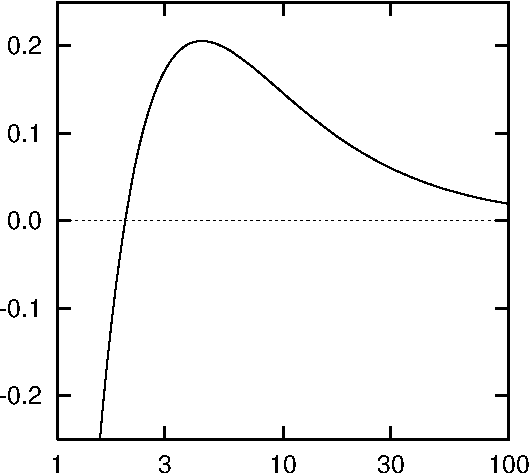
\includegraphics{AEIThorns_AHFinderDirect_Schw_EF_Theta_of_r}
\end{center}
\caption[Expansion $\Theta$ for $r = \text{constant}$ Surfaces
	 in an Eddington-Finkelstein slice
	 of the Unit-Mass Schwarzschild Spacetime]
	{
	This figure shows the expansion $\Theta$ for $r = \text{constant}$
	surfaces in an Eddington-Finkelstein slice of the unit-Mass
	Schwarzschild Spacetime.
	}
\label{AHFinderDirect/fig-Schwarzschild-EF-Theta(r)}
\end{figure}
%%%%%%%%%%%%%%%%%%%%%%%%%%%%%%%%%%%%%%%%

\end{description}

%%%%%%%%%%%%%%%%%%%%%%%%%%%%%%%%%%%%%%%%%%%%%%%%%%%%%%%%%%%%%%%%%%%%%%%%%%%%%%%%

\section{Monitoring \thorn{AHFinderDirect}'s Status}

There are two primary ways of monitoring what \thorn{AHFinderDirect}
is doing during a Cactus run: the \verb|BH_diagnostics| files and the
\verb|CCTK_INFO| messages written to the Cactus standard output:

The \verb|BH_diagnostics| files are described in detail in
section~\ref{AHFinderDirect/sect-parameters/BH-diagnostics-parameters}.
These files are written and ``flushed'' at each time step, so they're
always up-to-date.

During the apparent-horizon--finding process, \thorn{AHFinderDirect}
writes various \verb|CCTK_INFO| messages describing the convergence
of the iterative solution of the apparent horizon
equation~\ref{AHFinderDirect/eqn-horizon} on each processor.
In particular, if \verb|verbose_level| is set to
\verb|"algorithm highlights"| or a more verbose setting
(\cf{}~section~\ref{AHFinderDirect/sect-parameters/overall-parameters}),
then \thorn{AHFinderDirect} writes \verb|CCTK_INFO| messages like
these:
\begin{verbatim}
INFO (AHFinderDirect):    proc 0/horizon 1:it 1 r_grid=0.595 ||Theta||=1.1e-01
INFO (AHFinderDirect):    proc 0/horizon 1:it 2 r_grid=0.614 ||Theta||=7.2e-02
INFO (AHFinderDirect):    proc 0/horizon 1:it 3 r_grid=0.632 ||Theta||=2.9e-02
INFO (AHFinderDirect):    proc 0/horizon 1:it 4 r_grid=0.642 ||Theta||=9.9e-04
INFO (AHFinderDirect):    proc 0/horizon 1:it 5 r_grid=0.642 ||Theta||=7.9e-07
INFO (AHFinderDirect):    proc 0/horizon 1:it 6 r_grid=0.642 ||Theta||=7.2e-13
INFO (AHFinderDirect): AH 1/2: r=0.660716 at (0.000000,0.000000,1.127434)
INFO (AHFinderDirect): AH 1/2: area=338.0473838 m_irreducible=2.59330658
INFO (AHFinderDirect): writing h to "misner.h.t0.ah1.gp"
\end{verbatim}
Here \verb|r_grid| is a rough estimate of the mean radius of
the trial surface at each iteration, and \verb:||Theta||: is the
infinity-norm of $\Theta$, the left hand side of the apparent
horizon equation~\ref{AHFinderDirect/eqn-horizon} over the surface.
Once the apparent horizon has been found
(\verb:||Theta||: is sufficiently small), then \thorn{AHFinderDirect}
prints its mean radius,%%%
\footnote{%%%
	 Note that this may differ significantly from
	 the last iterations' estimated radius.  This
	 is because the mean radius printed during the
	 iterations is only a rough estimate (it's the
	 unweighted arithmetic mean of the radius at
	 all the horizon-surface grid points), while
	 the radius printed after the horizon is found
	 is a more accurate value (it's computed via
	 numerical integrals over the surface, taking
	 into account the induced metric).
	 }%%%
{} centroid position, area, and irreducible mass.

%%%%%%%%%%%%%%%%%%%%%%%%%%%%%%%%%%%%%%%%%%%%%%%%%%%%%%%%%%%%%%%%%%%%%%%%%%%%%%%%

\section{Visualization}
\label{AHFinderDirect/sect-visualization}

There are several ways to visualize \thorn{AHFinderDirect}'s output:

The simplest is to plot various quantities from the
\verb|BH_diagnostics| files (described in detail in
section~\ref{AHFinderDirect/sect-parameters/BH-diagnostics-parameters}).
For example, using gnuplot (\verb|http://www.gnuplot.info|), you can
plot a graph of the surface area of horizon \#4 as a function of
coordinate time, with the command
\begin{verbatim}
plot 'BH_diagnostics.ah4.gp' using 2:26 with points
\end{verbatim}
ygraph (\verb|http://www.aei.mpg.de/~pollney/ygraph/|) may also be
able to directly plot the \verb|BH_diagnostics| files.

Given a horizon-shape data file \verb|h.t105.h4.gp|, the gnuplot
command
\begin{verbatim}
splot 'h.t105.h4.gp' with lines
\end{verbatim}
will plot the $h(\text{angle})$ function, with the $x$ and $y$~axes
of the plot being the two ``unwrapped'' angular coordinates on $S^2$,
in degrees, and the $z$~axis being $h(\text{angle})$.  However,
in practice this usually isn't very informative.  Instead, you
probably want the gnuplot command
\begin{verbatim}
splot 'h.t105.h4.gp' using 4:5:6 with lines
\end{verbatim}
which will plot the 3-D shape of the apparent horizon surface.

The \verb|src/misc| directory of the \thorn{AHFinderDirect} source
code contains several perl scripts which are useful in visualizing
\thorn{AHFinderDirect} output.  In particular, the script \verb|select.plane|
selects a particular 2-D plane.  If you put this in your Unix path,
it can be used with a gnuplot command like
\begin{verbatim}
splot '<select.plane xy <h.t105.h4.gp' using 4:5 with lines
\end{verbatim}
to show the shape of an apparent horizon in the xy plane.%%%
\footnote{%%%
	 Note that this script isn't very smart: it doesn't
	 know about the \thorn{AHFinderDirect} local coordinate
	 origin.  That is, for example, if you select the $xy$
	 plane, you're selecting the \emph{global} $xy$ plane
	 ($z=0$).
	 }%%%

Another Visualization option is OpenDX (\verb|http://www.opendx.org/|).
Thomas Radke's has written some OpenDX macros
\program{ImportAHFinderDirectGnuplot.net}
and \program{ImportAHFinderDirectGnuplotPatch.net}
to import \thorn{AHFinderDirect} horizon-shape data files.  
These macros use a set of ``control files'' named \verb|*.dx|,
one per horizon, which \thorn{AHFinderDirect} (by default) writes
into the same directory as the main horizon--shape output files.
You can get these macros by anonymous CVS with the command
\begin{verbatim}
cvs -d :pserver:cvs_anon@cvs.aei.mpg.de:/numrelcvs \
     checkout AEIPhysics/Visualization/OpenDX
\end{verbatim}

Another Visualization option is to produce files in the standard
Xdmf~\cite{AHFinderDirect/Xdmf:web} file format which can be visualized for
example using VisIt~\cite{AHFinderDirect/VisIt:web}. Frank L\"offler has
written a python script \program{AH2xdmf.py}, which is included in this
thorn's code repository, which generates such files from
\thorn{AHFinderDirect}'s output from horizon shape files
\verb|h.t%d.ah%d.gp\|. Please see its help text for details.

%%%%%%%%%%%%%%%%%%%%%%%%%%%%%%%%%%%%%%%%%%%%%%%%%%%%%%%%%%%%%%%%%%%%%%%%%%%%%%%%

\section{Accuracy}

The apparent horizon positions are typically computed very accurately;
tests on Kerr spacetimes give typical errors of $10^{-4}m$ to $10^{-5}m$.

The various diagnostics printed to standard output and written to the
black hole diagnostics file(s), are typically computed to accuracies
on the order of a part per million or so.

Note, however, that the irreducible mass $m_{\text{e}}$
may differ considerably from the black hole's local mass or its
contribution to the slice's ADM mass.  For example, for Kerr spacetime
in Kerr-Schild coordinates,
$m_{\text{e}}/m_{\text{M}} = 0.949$, $0.894$, and $0.723$
for spin parameters $a \equiv J/m^2 = 0.6$, $0.8$, and $0.999$, respectively.
It would be better to (also) use the ``isolated horizons'' formalism of
\cite{AHFinderDirect/Dreyer-etal-2002-isolated-horizons};
at some point this thorn may be enhanced to do this.

%%%%%%%%%%%%%%%%%%%%%%%%%%%%%%%%%%%%%%%%%%%%%%%%%%%%%%%%%%%%%%%%%%%%%%%%%%%%%%%%

\section{Examples}
\label{AHFinderDirect/sect-examples}

There are a few example parameter files in the \code{par/} directory,
including Kerr initial data, Misner initial data, and Misner time-evolution
tests.  The \verb|Kerr-tiny.par| parameter file is close to a minimal
\thorn{AHFinderDirect} example:

\begin{verbatim}
# This parameter file sets up Kerr/Kerr-Schild initial data, then
# finds the apparent horizon in it.  The local coordinate system origin
# and the initial guess are both deliberately de-centered with respect
# to the black hole, to make this a non-trivial test for the apparent
# horizon finder.
#
# This parameter file is "tiny" in the sense that it sets only a
# small number of AHFinderDirect parameters.

# flesh
cactus::cctk_itlast = 0

ActiveThorns = "PUGH"
driver::ghost_size = 2
driver::global_nx = 31
driver::global_ny = 31
driver::global_nz = 19

ActiveThorns = "CoordBase CartGrid3D"
grid::domain = "bitant"
grid::avoid_origin = false
grid::type = "byspacing"
grid::dxyz = 0.2

ActiveThorns = "ADMBase ADMCoupling StaticConformal Spacemask CoordGauge Exact"
ADMBase::initial_lapse = "exact"
ADMBase::initial_shift = "exact"
ADMBase::initial_data = "exact"
ADMBase::lapse_evolution_method = "static"
ADMBase::shift_evolution_method = "static"
ADMBase::metric_type = "physical"
Exact::exact_model = "Kerr/Kerr-Schild"
Exact::Kerr_KerrSchild__mass = 1.0
Exact::Kerr_KerrSchild__spin = 0.6

########################################

ActiveThorns = "IOUtil"
IOUtil::parfile_write = "no"

########################################

ActiveThorns = "SphericalSurface"
ActiveThorns = "AEILocalInterp PUGHInterp PUGHReduce AHFinderDirect"
AHFinderDirect::h_base_file_name     = "Kerr-tiny.h"

AHFinderDirect::N_horizons = 1
AHFinderDirect::origin_x[1] = 0.5
AHFinderDirect::origin_y[1] = 0.7
AHFinderDirect::origin_z[1] = 0.0

AHFinderDirect::initial_guess_method[1] = "coordinate sphere"
AHFinderDirect::initial_guess__coord_sphere__x_center[1] = -0.2
AHFinderDirect::initial_guess__coord_sphere__y_center[1] =  0.3
AHFinderDirect::initial_guess__coord_sphere__z_center[1] =  0.0
AHFinderDirect::initial_guess__coord_sphere__radius[1] = 2.0
\end{verbatim}

%%%%%%%%%%%%%%%%%%%%%%%%%%%%%%%%%%%%%%%%%%%%%%%%%%%%%%%%%%%%%%%%%%%%%%%%%%%%%%%%

\section{Surfaces of Constant Expansion}

Surfaces of Constant Expansion (CE surfaces) are introduced in
\cite{AHFinderDirect/Schnetter03a} as a generalisation of
apparent horizons (AH).  On an AH surface, the expansion is zero
everywhere.  On a CE surfaces, the expansion is still everywhere the
same, but it need not be zero.  CE surfaces are also a generalisation
of Constant Mean Curvature surfaces (CMC surfaces); both are identical
when the extrinsic curvature vanishes.  As described in
\cite{AHFinderDirect/Schnetter03a}, it is likely that CE
surfaces foliate the spacelike hypersurface outside of some interior
region.  This interior region is inside the common apparent horizon,
if it exists.

CE surfaces can give some insight into the spacetime, because they can
be used to analyse the part of the spacelike hypersurface ``between
the horizons and infinity''.  Most notably, they can be used to look
at the region where a common horizon is about to (or believed to)
form.  Similarly, one can use them for collapsing stars where an
apparent horizon has not yet formed.

%%%%%%%%%%%%%%%%%%%%%%%%%%%%%%%%%%%%%%%%%%%%%%%%%%%%%%%%%%%%%%%%%%%%%%%%%%%%%%%%

\section{Pretracking}

Apparent horizon pretracking is introduced in
\cite{AHFinderDirect/Schnetter03a}.  This is an application
of CE surfaces.  Even when there is no common horizon, there are still
common CE surfaces surrounding multiple black holes.  Pretracking
consists of tracking in time the smallest common CE surface that can
be found.  It is reasonable to believe that this surface will evolve
into the common horizon at the time where this common horizon begins
to exist.  The expansion of this smallest CE surface is also an
indication of how close the spacelike hypersurface is to having a
common apparent horizon.

%%%%%%%%%%%%%%%%%%%%%%%%%%%%%%%%%%%%%%%%%%%%%%%%%%%%%%%%%%%%%%%%%%%%%%%%%%%%%%%%

\section{How \thorn{AHFinderDirect} Works}
\label{AHFinderDirect/sect-how-ahfinderdirect-works}

\thorn{AHFinderDirect} uses the apparent horizon
(henceforth \defn{horizon}) finding algorithm of
\cite{AHFinderDirect/Thornburg95},
modified slightly to work with $g_\ij$ and $K_\ij$ on a Cartesian ($xyz$)
grid.  The algorithm is described in detail in
\cite{AHFinderDirect/Thornburg2003:AH-finding}.

%%%%%%%%%%%%%%%%%%%%%%%%%%%%%%%%%%%%%%%%

\subsection{General Description of the Algorithm}

As described above, I parameterizes the horizon shape by
$r = h(\text{angle})$ for some single-value function $h: S^2 \to \Re^+$.
The apparent horizon equation~\eqref{AHFinderDirect/eqn-horizon}
then becomes a 2-D elliptic PDE on $S^2$ for the function $h$.  I finite
difference this in angle to obtain a system of simultaneous nonlinear
algebraic equations for $h$ at the angular grid points, and solve this
system of equations by a global Newton's method (or a variant with
improved convergence).

Computationally, this algorithm has 3 main parts:
\begin{itemize}
\item	Computation of the ``horizon function'' $\Theta(h)$ given a trial
	surface defined by a trial horizon shape function $h$.  This is
	done by interpolating the Cactus geometry fields $g_\ij$ and
	$K_\ij$ (and optionally $\psi$) from the 3-D $xyz$ grid to the
	(2-D set of) trial-horizon-surface grid points (also computing
	$\partial_k g_\ij$ in the interpolation process), then doing
	all further computations with angular grid functions defined
	solely on $S^2$ (\ie{} at the horizon-surface grid points).
\item	Computation of the Jacobian matrix $\Jac[\Theta(h)]$ of $\Theta(h)$.
	This thorn incorporates the \defn{symbolic differentiation} technique
	described in \cite{AHFinderDirect/Thornburg95},
	so this computation is quite fast.  The Jacobian is a highly
	sparse matrix; \thorn{AHFinderDirect} has code to store it
	as either a dense matrix (for debugging purposes), or a sparse
	matrix (the default).  Which option is used is determined by
	a compile-time configuration in \verb|src/include/config.h|.
\item	Solving the nonlinear equations $\Theta(h) = 0$ by a global
	Newton's method or a variant.  How this is done depends on how
	the Jacobian is stored.  At present,
	\begin{itemize}
	\item	If \thorn{AHFinderDirect} is configured to store the
		Jacobian as a dense matrix, then LAPACK is used to solve
		the linear equations.
	\item	If \thorn{AHFinderDirect} is configured to store the
		Jacobian as a sparse matrix, then an
		incomplete-$\sf LU$-decomposition--conjugate-gradient
		solver is used.
	\end{itemize}
	By default only the sparse-matrix code is configured, so LAPACK
	isn't used and there's no need to link with the LAPACK library.
\end{itemize}

%%%%%%%%%%%%%%%%%%%%%%%%%%%%%%%%%%%%%%%%

\subsection{The Multipatch System}
\label{AHFinderDirect/sect-multipatch-system}

Perhaps the most unusual feature of \thorn{AHFinderDirect} is the
``multipatch'' system used to cover $S^2$ without coordinate singularities.
In general there are 6~patches, one each covering a neighborhood of
the $\pm z$, $\pm x$, and $\pm y$ axes, but this may be reduced in
the presence of suitable symmetries.  For example,
figure~\ref{AHFinderDirect/fig-3patch}
on page~\pageref{AHFinderDirect/fig-3patch} shows a system
of 3~patches covering the $+xyz$~octant of $S^2$.  This would be
suitable for finding an apparent horizon with mirror symmetry about
the (local) $z=0$~plane, and either 90~degree periodic rotation symmetry
about the (local) $z$~axis, or mirror symmetry about each of the (local)
$x$~and $y$~axes.

\begin{figure}[htbp]
\begin{center}
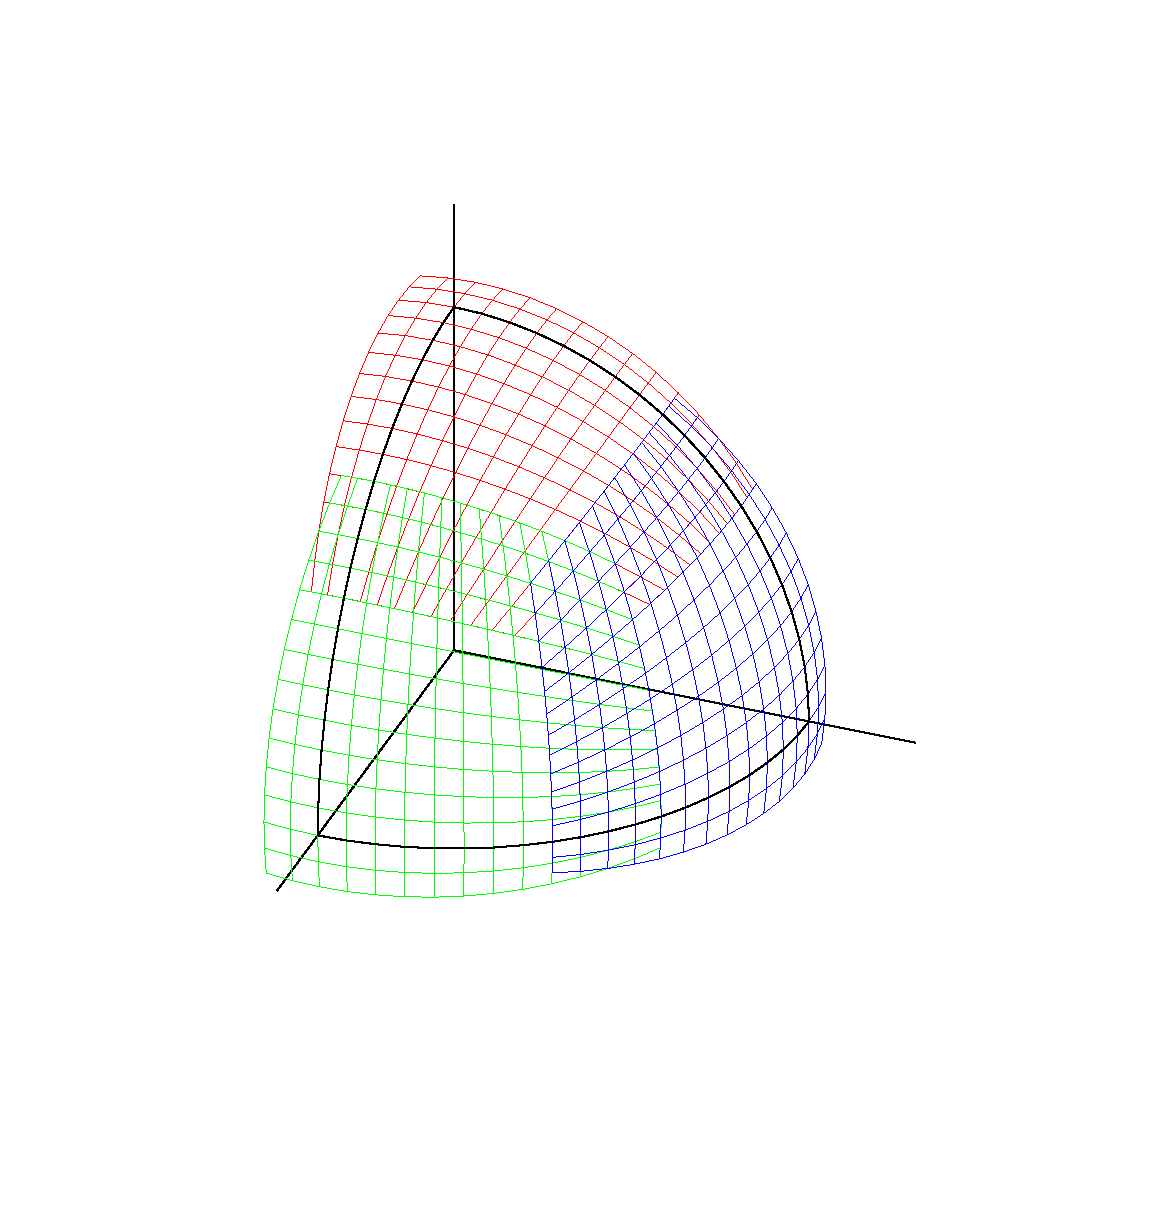
\includegraphics{AEIThorns_AHFinderDirect_3patch}
\end{center}
\caption[Illustration of the Multipatch System]
	{
	This figure shows a multipatch system covering the
	$(+,+,+)$~octant of the unit sphere~$S^2$ with 3~patches.
	The angular resolution is 5~degrees.  Notice that the
	patches overlap by several ``ghost zone'' grid points.
	}
\label{AHFinderDirect/fig-3patch}
\end{figure}

To allow easy angular finite differencing within the patch system,
each patch is extended beyond its nominal extent by a ``ghost zone''%%%
\footnote{%%%
	 Note that this terminology differs somewhat
	 from that used by Cactus in general; Cactus
	 would call these ``patch zones'' or ``symmetry
	 zones''.
	 }%%%
{} (2~grid points wide in figure~\ref{AHFinderDirect/fig-3patch}).
Angular grid function values in the ghost zone can be obtained by
interpatch interpolation%%%
\footnote{%%%
	 Due to the way the patch coordinates are defined,
	 adjacent patches always share a common ``perpendicular''
	 angular coordinate, so only 1-D interpolation
	 is needed here.
	 }%%%
{} or by applying symmetry operations.  Once this is done, then angular
finite differencing within the nominal extent of each patch can proceed
normally, ignoring the patch boundaries.  \thorn{AHFinderDirect} can
be configured at compile time to use either 2nd~order or 4th~order
angular finite differencing (3~point or 5~point angular molecules);
the default is 4th~order (5~point).  This is configured at compile time
in \verb|src/include/config.h|.

By default \thorn{AHFinderDirect} will automagically choose a patch
system type for each apparent horizon searched for, based on the local
coordinate origin and the symmetries implicit in the Cactus grid type.
This generally works well, but if desired you can instead manually
specify the patch system type, the angular resolution, the width of
the ghost zones, etc.  See the \verb|param.ccl| file for details.

%%%%%%%%%%%%%%%%%%%%%%%%%%%%%%%%%%%%%%%%

\subsection{Other Software Used}

\thorn{AHFinderDirect}'s \verb|src/sparse-matrix/| directory contains
various sparse-matrix libraries, which have their own copyrights and
licensing terms:

The \verb|src/sparse-matrix/umfpack/| directory contains a subset of the
files in UMFPACK version 4.0 (11.Apr.2002).  This code is
copyright~(\copyright)~2002 by Timothy A. Davis, and is subect to the
UMFPACK License:

\begin{verbatim}
Your use or distribution of UMFPACK or any modified version of
UMFPACK implies that you agree to this License.

THIS MATERIAL IS PROVIDED AS IS, WITH ABSOLUTELY NO WARRANTY
EXPRESSED OR IMPLIED.  ANY USE IS AT YOUR OWN RISK.

Permission is hereby granted to use or copy this program, provided
that the Copyright, this License, and the Availability of the original
version is retained on all copies.  User documentation of any code that
uses UMFPACK or any modified version of UMFPACK code must cite the
Copyright, this License, the Availability note, and "Used by permission."
Permission to modify the code and to distribute modified code is granted,
provided the Copyright, this License, and the Availability note are
retained, and a notice that the code was modified is included.  This
software was developed with support from the National Science Foundation,
and is provided to you free of charge.
\end{verbatim}

%%%%%%%%%%%%%%%%%%%%%%%%%%%%%%%%%%%%%%%%%%%%%%%%%%%%%%%%%%%%%%%%%%%%%%%%%%%%%%%%

\section{Other Related Thorns}

If you're interested in \thorn{AHFinderDirect}, you might also be
interested in some other related thorns:

\begin{description}
\item[\thorn{EHFinder}] (in the \arrangement{AEIDevelopment} arrangement)
	was written by Peter Diener, and finds the {\em event\/} horizon(s)
	in a numerically computed spacetime.  It's described in detail in
	the paper~\cite{AHFinderDirect/Diener03a}.
\item[\thorn{AHFinder}] (in the \arrangement{CactusEinstein} arrangement)
	was written by Miguel Alcubierre, and includes two different
	algorithms for finding apparent horizons, a minimization method
	and a ``fast flow'' method based on \cite{AHFinderDirect/Gundlach97a}.
	Unfortunately, both methods are very slow in practice.
\item[\thorn{TGRapparentHorizon2D}] (in the \arrangement{TAT} arrangement)
	was written by Erik Schnetter, and is another apparent horizon
	finder.  It uses methods very similar to this thorn, and (like
	this thorn) is very fast and accurate.  However, it's no longer
	under active development.  It's described in detail in the
	papers~\cite{AHFinderDirect/Schnetter02a}
	and~\cite{AHFinderDirect/Schnetter03a}.
\item[\thorn{AHFinderDirect} (\cvsplace{Erik} branch)]
      (in the \arrangement{AEIThorns} arrangement)\\
	Erik Schnetter has added a number of new features to
	\thorn{AHFinderDirect} on a CVS branch with the tag \cvsplace{Erik},
	including horizon pretracking (to locate places where horizons
	are about to form), and the ability to find constant-expansion
	and constant-mean-curvature surfaces specified by their areal radius.
	We hope to integrate these into the main \thorn{AHFinderDirect}
	branch during the summer of 2004.
\end{description}

%%%%%%%%%%%%%%%%%%%%%%%%%%%%%%%%%%%%%%%%%%%%%%%%%%%%%%%%%%%%%%%%%%%%%%%%%%%%%%%%

\section{Acknowledgments}

I thank Peter Diener, Ian Hawke, and Erik Schnetter for many valuable
conversations.  I think Thomas Radke for his work on the new interpolators.
I thank the whole Cactus crew for a great infrastructure!

Erik Schnetter originally implemented a number of improvements to
this thorn, notably the \thorn{SphericalSurface} interface and the
new features in the \cvsplace{Erik} branch.

I thank the Alexander von Humboldt foundation and the AEI visitors'
and postdoctoral fellowships programs for financial support.

%%%%%%%%%%%%%%%%%%%%%%%%%%%%%%%%%%%%%%%%%%%%%%%%%%%%%%%%%%%%%%%%%%%%%%%%%%%%%%%%

% make LaTeX read in AHFinderDirect.bbl produced by bibtex
\bibliography{AHFinderDirect}

%%%%%%%%%%%%%%%%%%%%%%%%%%%%%%%%%%%%%%%%%%%%%%%%%%%%%%%%%%%%%%%%%%%%%%%%%%%%%%%%

% Do not delete next line
% END CACTUS THORNGUIDE

\end{document}
